\begin{lstlisting}
习题1.3第20题
习题1.4第3,4,6,9,11题
\end{lstlisting}
\begin{exercise}
\begin{figure}[H]
\centering
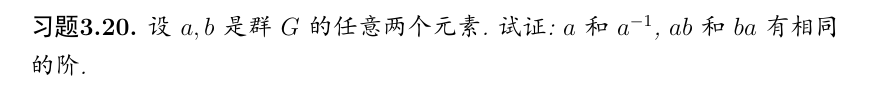
\includegraphics[width=\textwidth]{1-hw3-2025032510.png}
% \caption{}
\label{}
\end{figure}
\end{exercise}
\begin{proof}
若 $O(a)=n$,则 $a^{n}=e$,$e=(a^{-1})^{n}$. 故 $O(a^{-1})\leq n=O(a)$. 同理 $O(a)\leq O(a^{-1})$. 故 $O(a)=O(a^{-1})$.

若 $O(ab)=n$,则
\[
(ab)^{n}=\underbrace{ ab\cdot ab\cdot\dots \cdot ab }_{ n\text{ times} }=e
\]
左乘 $a^{-1}$,再右乘 $a$ 得到
\[
\underbrace{ ba\cdot ba\cdot\dots \cdot ba }_{ n\text{ times} }=a^{-1}a=e
\]
于是 $O(ba)\leq O(ab)$,同理 $O(ab)\leq O(ba)$,因此 $O(ab)=O(ba)$.

\end{proof}

\begin{note}
以后我们用 $\lvert x \rvert$ 表示 $\lvert \left< x \right> \rvert$,即 $x$ 的阶.
\end{note}
\begin{exercise}
\begin{figure}[H]
\centering
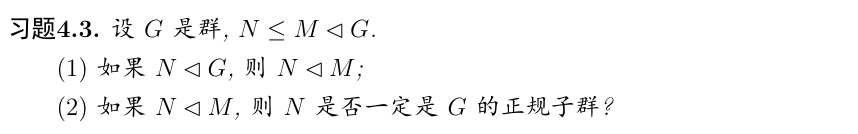
\includegraphics[width=\textwidth]{2-hw3-2025032510.png}
% \caption{}
\label{}
\end{figure}
\end{exercise}
(1) 若 $N\lhd G$,则 $\forall g\in G\supset M$,有 $gN=Ng$,显然 $N\lhd M$.

(2) 不一定,比如
\[
H_1\coloneqq\{ e, (12)(34) \}\lhd H_2\coloneqq \{ e,(12)(34),(13)(24),(14)(23) \}\lhd S_4
\]
但是 $H_1\centernot{\lhd}S_4$.

\begin{exercise}
\begin{figure}[H]
\centering
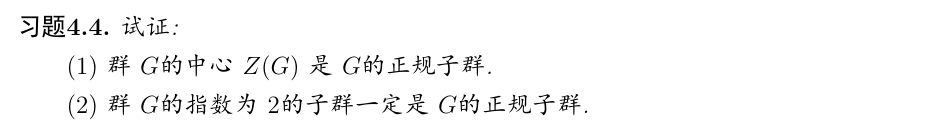
\includegraphics[width=\textwidth]{3-hw3-2025032510.png}
% \caption{}
\label{}
\end{figure}
\end{exercise}
\begin{proof}
(1)
\[
Z(G)\coloneqq \{ g\in G:\forall h\in G,ghg^{-1}=h \}
\]
Check that $\forall g\in G$,
\[
gZ(G)g^{-1}=Z(G)
\]
Fix $g$, then for any $h\in Z(G)$,
\[
ghg^{-1}=h\in Z(G)
\]
Therefore $Z(G)\lhd G$.

(2)
If $H\leq G$ with $[G:H]=2$, then $G$ can be split to two orbit
\[
G=H\sqcup gH=H\sqcup Hg,\qquad \text{for any }g\not\in H
\]
Then the left and right cosets of $g$ are the same.

For any given $g_1\in G$, check that $g_1Hg_1^{-1}=H$.

If $g_1\in H$, then $g_1Hg_1 ^{-1}=H$. If $g_1\not\in G$, then $g_1H=Hg_1$. Therefore $H\lhd G$.

\end{proof}

\begin{exercise}
\begin{figure}[H]
\centering
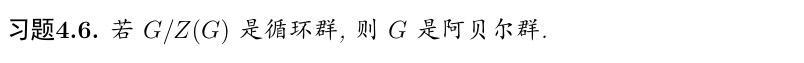
\includegraphics[width=\textwidth]{4-hw3-2025032510.png}
% \caption{}
\label{}
\end{figure}
\end{exercise}
\begin{proof}
\[
Z(G)\coloneqq \{ g\in G :\forall h\in G,ghg^{-1}=h\}
\]
Since $G/Z(G)$ is cyclic, then
\[
G/Z(G)=\{ Z(G),gZ(G),\dots,g^{m}Z(G) \}
\]
for any nontrivial $g\in G$.

Fix $g\in G$, check that $ghg^{-1}=h,\forall h\in G$.

We know that $h$ must lie in $g^{r}Z(G)$ for some $0\leq r\leq m$. Then $h=g^{r}h'$ for some $h'\in Z(G)$. Thus
\[
ghg^{-1}=g\cdot g^{r}h'\cdot g^{-1}\overset{ h'\in Z(G) }{ = }g^{r+1}\cdot g^{-1}h'=g^{r}h'=h
\]
Therefore $G$ is Abel.

\end{proof}

\begin{exercise}
\begin{figure}[H]
\centering

\includegraphics[width=\textwidth]{5-hw3-2025032510.png}
% \caption{}
\label{}
\end{figure}
\end{exercise}
\[
Z(\mathrm{GL}_n(\mathbb{R}))=\{ \mathrm{diag}\{ \lambda_1,\lambda_2,\dots,\lambda _n \}:\lambda _k\in \mathbb{R}^{\times},k=1,2,\dots,n \}
\]
\[
\mathrm{O}_{2}(\mathbb{R})\coloneqq \{ A\in \mathrm{GL}_2(\mathbb{R}) :AA^{T}=A^{T}A=I\}
\]
\[
Z(\mathrm{O}_{2}(\mathbb{R}))=\pm I
\]
\[
\mathrm{SO}_{3}(\mathbb{R})\coloneqq \{ A\in \mathrm{GL}_{3}(\mathbb{R}):AA^{T}=A^{T}A=I,\det A=1 \}
\]
\[
Z(\mathrm{SO}_{3}(\mathbb{R}))=I
\]
\[
\mathrm{SU}_{2}(\mathbb{C})\coloneqq \mathrm{U}(n)\cap \mathrm{SL}_2(\mathbb{C})=\{ \begin{pmatrix}
\alpha & \beta \\
-\overline{\beta} & \overline{\alpha} 
\end{pmatrix}:\alpha,\beta\in \mathbb{C},\lvert \alpha \rvert ^2+\lvert \beta \rvert ^2=1 \}
\]
Denote that
\[
A=\begin{pmatrix}
\alpha_1 & \beta_1 \\
-\overline{\beta}_{1} & \overline{\alpha}_{1}
\end{pmatrix},\qquad B=\begin{pmatrix}
\alpha_2 & \beta_2 \\
-\overline{\beta}_{2} & \overline{\alpha}_{2}
\end{pmatrix}
\]
Then
\[
AB=\begin{pmatrix}
\alpha_1\alpha_2-\beta_1\overline{\beta}_{2} & \alpha_1\beta_2+\beta_1\overline{\alpha}_{2} \\
-\alpha_2\overline{\beta}_{1}-\overline{\alpha}_{1}\overline{\beta}_{2} & -\overline{\beta}_{1}\beta_2+\overline{\alpha}_{1}\overline{\alpha}_{2}
\end{pmatrix}
\]
\[
BA=\begin{pmatrix}
\alpha_2\alpha_1-\beta_2\overline{\beta}_{1} & \alpha_2\beta_1+\beta_2\overline{\alpha}_{1} \\
-\alpha_1\overline{\beta}_{2}-\overline{\alpha}_{2}\overline{\beta}_{1} & -\overline{\beta}_{2}\beta_1+\overline{\alpha}_{2}\overline{\alpha}_{1}
\end{pmatrix}
\]
Thus
\[
\beta_2\overline{\beta}_{1}=\beta_1\overline{\beta}_{2},\qquad \alpha_1\beta_2+\beta_1\overline{\alpha}_{2}=\alpha_2\beta_1+\beta_2\overline{\alpha}_{1},\qquad \forall \alpha_2,\beta_2\in \mathbb{C}
\]
Then
\[
\beta_1=0,\qquad \alpha_1-\overline{\alpha}_{1}=0\Rightarrow\alpha_1\in \mathbb{R}
\]
Since $\lvert \alpha_1 \rvert ^2+\lvert \beta_1 \rvert ^2=1$, we have $\alpha_1=\pm1$. Then
\[
Z(\mathrm{SU}_{2}(\mathbb{C}))=\pm I
\]
\begin{exercise}
\begin{figure}[H]
\centering
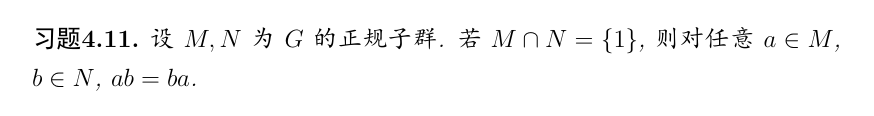
\includegraphics[width=\textwidth]{6-hw3-2025032510.png}
% \caption{}
\label{}
\end{figure}
\end{exercise}
\begin{proof}
Since $M\lhd G,N\lhd G$, for any $g\in G$, we have
\[
gMg^{-1}=M,\qquad gNg^{-1}=N
\]
Then for any $a\in M, b\in N$,
\[
a\underbrace{ ba^{-1}b^{-1} }_{ =a'\in M }=a\cdot a'\in M
\]
And
\[
\underbrace{ aba^{-1} }_{ =b'\in N }b^{-1}=b'\cdot b^{-1}\in N
\]
Thus
\[
aba^{-1}b^{-1}\in M\cap N=\{ 1 \}\implies ab=ba,\forall a\in M,b\in N
\]
\end{proof}
